% ===================================================================
% FILE: Lezione6.tex
% ===================================================================

\part{Lezione 22 (10/11/2025) }

\section{Mergesort }
Mergesort è un algoritmo di ordinamento basato su Divide et Impera.
\begin{definition}[Mergesort: Paradigma D\&I]
    \begin{itemize}
        \item \textbf{DIVIDE}: Divide l'array $A[p..r]$ in due metà, $A[p..q]$ e $A[q+1..r]$, dove $q = \lfloor (p+r)/2 \rfloor$.
        \item \textbf{IMPERA}: Ordina ricorsivamente le due metà chiamando \texttt{Mergesort(A, p, q)} e \texttt{Mergesort(A, q+1, r)}.
        \item \textbf{COMBINE}: Combina (fonde) i due sottoarray ordinati $A[p..q]$ e $A[q+1..r]$ in un unico array ordinato $A[p..r]$ tramite la procedura \texttt{Merge(A, p, q, r)}.
    \end{itemize}
\end{definition}

\subsection{Pseudocodice Mergesort}
\begin{algorithmic}[1]
    \Procedure{Mergesort}{A, p, r}
        \If{$p < r$}
            \State $q = \lfloor (p+r)/2 \rfloor$ \Comment{DIVIDE }
            \State \Call{Mergesort}{A, p, q} \Comment{IMPERA }
            \State \Call{Mergesort}{A, q+1, r} \Comment{IMPERA }
            \State \Call{Merge}{A, p, q, r} \Comment{COMBINE }
        \EndIf
    \EndProcedure
\end{algorithmic}

\begin{explanation}{Logica Mergesort}
Divide et Impera puro:
\begin{enumerate}
    \item \textbf{Divide}: Calcola il punto medio $q$.
    \item \textbf{Impera}: Due chiamate ricorsive su metà array.
    \item \textbf{Combine}: La procedura \texttt{Merge} unisce i risultati.
\end{enumerate}
\end{explanation}

\subsection{Procedura Merge }

\begin{observation}[Procedura Merge]
    La procedura \texttt{Merge} fonde due sottoarray contigui $A[p..q]$ e $A[q+1..r]$, che si assumono \textbf{già ordinati}.
    Ha complessità \textbf{Lineare} $T(n) = \Theta(n)$, dove $n = r-p+1$.
    Utilizza due array di appoggio, $L$ e $R$, e due "sentinelle" ($\infty$) per evitare controlli sull'indice.
\end{observation}

\begin{algorithmic}[1]
    \Procedure{Merge}{A, p, q, r}
        \State $n_1 = q - p + 1$ \Comment{Dim. primo sottoarray }
        \State $n_2 = r - q$ \Comment{Dim. secondo sottoarray }
        \State Crea array $L[1..n_1+1]$ e $R[1..n_2+1]$

        \Comment{Copia i dati negli array di appoggio}
        \For{$i = 1 \to n_1$}
            \State $L[i] = A[p + i - 1]$
        \EndFor
        \For{$j = 1 \to n_2$}
            \State $R[j] = A[q + j]$
        \EndFor

        \State $L[n_1 + 1] = +\infty$ \Comment{Sentinella }
        \State $R[n_2 + 1] = +\infty$ \Comment{Sentinella }

        \State $i = 1$ \Comment{Indice per $L$ }
        \State $j = 1$ \Comment{Indice per $R$ }

        \Comment{Fondi L e R nell'array A}
        \For{$k = p \to r$}
            \If{$L[i] \le R[j]$}
                \State $A[k] = L[i]$
                \State $i = i + 1$
            \Else
                \State $A[k] = R[j]$
                \State $j = j + 1$
            \EndIf
        \EndFor
    \EndProcedure
\end{algorithmic}

\begin{explanation}{Procedura Merge}
Fonde due sotto-array ordinati in uno solo.
\begin{itemize}
    \item Usa due array di appoggio $L$ e $R$.
    \item Le "sentinelle" ($\infty$) evitano di dover controllare se un array è finito mentre si confrontano gli elementi.
    \item Complessità $\Theta(n)$.
\end{itemize}
\end{explanation}

\subsection{Analisi Complessità Mergesort }

\begin{definition}[Analisi Mergesort: Ricorrenza]
    \textbf{Equazione di Ricorrenza:}
    $a=2$ sottoproblemi, $n/b = n/2$.
    $f(n) = D(n) \text{ (cost.)} + C(n) \text{ (Merge)} = \Theta(1) + \Theta(n) = \Theta(n)$.
    $$ T(n) = \begin{cases} \Theta(1) & \text{se } n = 1 \text{ } \\ 2T(n/2) + \Theta(n) & \text{se } n > 1 \text{ } \end{cases} $$
\end{definition}

\textbf{Soluzione 1: Albero di Ricorsione}
L'albero di ricorsione mostra il costo $f(n_i)$ ad ogni livello.
    % Grafico sostituito con immagine esterna su richiesta
    % \includegraphics[width=\textwidth]{img/nome_immagine.png} 
    \includegraphics[width=\textwidth]{img/albero_mergesort.png}
Il costo per ogni livello è $cn$. L'albero ha $\log_2 n$ livelli.
Il costo totale è $cn \cdot \log_2 n = \Theta(n \log n)$.
\begin{observation}[Analisi Mergesort: Metodo Iterativo]
    \textbf{Soluzione 2: Metodo Iterativo (Sostituzione)}
    $T(n) = 2T(n/2) + cn$
    $T(n) = 2(2T(n/4) + c(n/2)) + cn = 4T(n/4) + cn + cn = 4T(n/4) + 2cn$
    $T(n) = 4(2T(n/8) + c(n/4)) + 2cn = 8T(n/8) + cn + 2cn = 8T(n/8) + 3cn$
    ... dopo $i$ passi...
    $T(n) = 2^i T(n/2^i) + i \cdot cn$
    Ci si ferma al caso base $n/2^i = 1 \implies i = \log_2 n$.
    $T(n) = 2^{\log_2 n} T(1) + (\log_2 n) \cdot cn$
    $T(n) = n \cdot \Theta(1) + cn \log_2 n = \Theta(n \log n)$.
\end{observation}


\begin{observation}[Complessità in Spazio: Mergesort]
    Mergesort \textbf{non} ordina "in loco", poiché richiede $\Theta(n)$ spazio ausiliario per gli array $L$ e $R$ ad ogni chiamata di \texttt{Merge}.
\end{observation}

\subsection{Esempio: Albero delle Chiamate }
Per $A[1..7]$, l'ordine delle chiamate ricorsive è:
\begin{center}
    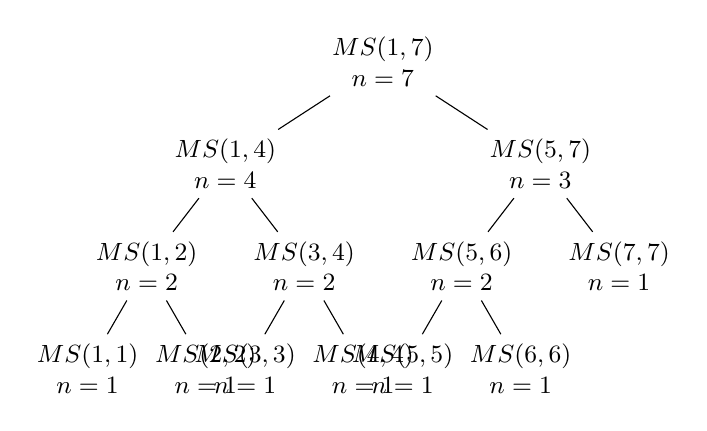
\begin{tikzpicture}[
        level distance=1.3cm,
        level 1/.style={sibling distance=4cm},
        level 2/.style={sibling distance=2cm},
        level 3/.style={sibling distance=1.5cm},
        every node/.style={align=center, font=\small}
        ]
        \node {$MS(1,7)$ \\ $n=7$ }
        child {node {$MS(1,4)$ \\ $n=4$ }
        child {node {$MS(1,2)$ \\ $n=2$ }
        child {node {$MS(1,1)$ \\ $n=1$ }}
        child {node {$MS(2,2)$ \\ $n=1$ }}
        }
        child {node {$MS(3,4)$ \\ $n=2$ }
        child {node {$MS(3,3)$ \\ $n=1$ }}
        child {node {$MS(4,4)$ \\ $n=1$ }}
        }
        }
        child {node {$MS(5,7)$ \\ $n=3$ }
        child {node {$MS(5,6)$ \\ $n=2$ }
        child {node {$MS(5,5)$ \\ $n=1$ }}
        child {node {$MS(6,6)$ \\ $n=1$ }}
        }
        child {node {$MS(7,7)$ \\ $n=1$ }}
        };
    \end{tikzpicture}
\end{center}

\newpage
